\section{Introduction}
\section{Synopsis of the Standard Model}
The Standard Model of particle physics is a description of the fundamental constituents of the Universe, as well as the interactions between them.
The model is composed of two main groups of particles, namely the fermions, which possess half-integer quantum spin, and make up all of the 
matter within the Universe, and the gauge bosons, which are of integer quantum spin, and are responsible for mediating forces between the fermions.\\
\\
The fermions can be further classified into two categories of fundamental particles known as quarks and leptons. There exist six distinct 'flavours' of quarks, which are
ascribed the names up, down, charm, strange, top and bottom, denoted, $u, d, c, s, t$ and $b$ respectively. These are grouped into three 'generations' based on their electromagnetic charge
and mass. Free quarks are never observed in nature due to a principle known as quark confinement, which mandates that these particles (and their antiparticles) should exist as bound states known as baryons and mesons
(which are collectively referred to as hadrons). Quarks can interact via all of the abovementioned forces. The leptons are grouped similarly by flavour, with each generation containing a negatively charged particle and a corresponding neutrino
whose electromagnetic charge is zero, and is, to a large extent, massless. The three different flavours of leptons, in ascending order of their masses, are the electron, muon and tau, denoted $e^{-}, \mu^{-}$, and $\tau^{-}$ respectively. The charged leptons
can only partake in electromagnetic and weak interactions while the neutrinos can only participate in weak processes.\\
\\
Three of the four fundamental forces of nature (i.e. the strong, electromagnetic and weak forces) are accounted for in the Standard Model, as evident through the presence of vector (spin 1) gauge bosons such as the gluon ($g$), photon ($\gamma$), and charged $W$ and neutral $Z$ bosons, 
which mediate the aforementioned forces respectively. The model also describes a spin-0 particle, known as the Higgs boson, which, through the mechanism of spontaneous symmetry breaking, is responsible for the Standard Model particles acquiring their mass. A spin-2, massless boson, known as the graviton
has also been hypothesised as a mediator of the gravitational force. However, there is no experimental evidence of this to date. Figure \ref{StandardModel} provides a visual summary of the model that has been described above.\\
\\
\begin{figure}[H]
    \centering
    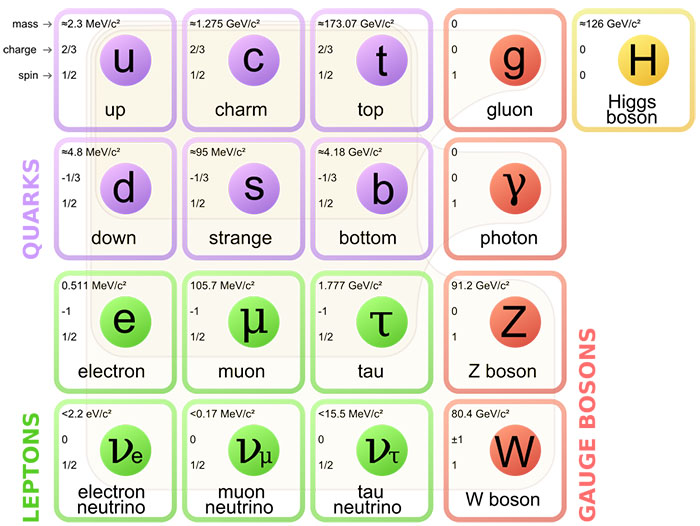
\includegraphics[scale = 0.4]{StandardModel.jpg}
    \caption{The particles of the Standard Model, grouped based on their quantum spin into gauge bosons and fermions (particles that make up all matter).The fermions are further divided into quarks and leptons which are fundamental, and can partake in various interactions that are mediated by the gauge bosons corresponding to each of the three fundamental forces described by the model. The Higgs boson is also included, and is responsible for all of the particles acquiring their mass.}
    \label{StandardModel}
\end{figure}
Despite providing a comprehensive description of the fundamental components of nature and the force acting between these, the Standard Model is subject to numerous limitations, the most prominent of which is its inability to account for the gravitational force. Furthermore, the nature of dark matter and dark energy, which account for
a large proportion of the matter in the Universe, is not fully understood, and remains an area of ongoing research. A more subtle limitation, however, pertains to a phenomenon known as CP violation and the absence of experimental evidence of this in the strong force, despite being theoretically permissible by the quantum field theory of this force,
known as quantum chromodynamics (QCD). This is known as the Strong CP problem and forms the basis for motivating particles such as the axion, as well as Axion-Like Particles (ALPs), both of which are described in further detail in the sections that follow.
\section{CP Violation}
The principle of symmetry (i.e. the invariance of a physical system under a transformation) is significant in the study of particle physics. Two symmetries that are of particular interest are those of charge conjugation, denoted $C$, and parity, denoted $P$. Charge conjugation is a transformation wherein particles within a physical system are interchanged with
their antiparticles, as demonstrated in Figure \ref{ChargeConjugation}, while parity refers to the inversion of spatial coordinates of a physical system, as illustrated in Figure \ref{ParityTransformation} below. 
\\
\\
The combination of the abovementioned transformations is referred to as $CP$, and its violation is of particular interest as it provides a possible explanation for the abundance of matter over antimatter in the Universe. CP symmetry has been observed to be preserved in electromagnetic interactions, whilst being violated in weak interactions, as demonstrated by 
a study of the decay of neutral kaons by Cronin and Fitch in 1964. While the theory of QCD permits the violation of this symmetry in the strong force, there is no experimental evidence of processes that violate this symmetry. This is referred to as the Strong CP problem, and is essential for the theoretical motivation behind axions and ALPs.
\begin{figure}[H]
    \centering
    \begin{subfigure}{0.5\textwidth}
        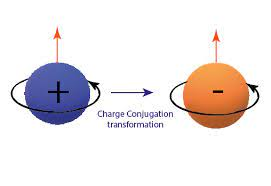
\includegraphics[]{ChargeConjugation.jpg}
        \caption{The charge conjugation transformation $C$, which interchanges particles in a physical system with their corresponding antiparticles.}
        \label{ChargeConjugation}
    \end{subfigure}
    \hfill
    \begin{subfigure}{0.7\textwidth}
        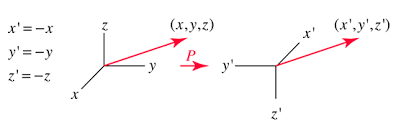
\includegraphics[]{ParityTransformation.png}
        \caption{An illustration of the parity transformation $P$, corresponding
        to the inversion of spatial coordinates in a physical system}
        \label{ParityTransformation}
    \end{subfigure}
    \hfill
\end{figure}
\subsection{The Strong CP Problem}\label{StrongCPProb}
The theoretically permissible nature of CP violation in the strong force is evident within the QCD Lagrangian, which can be written in the following form:
\begin{equation}\label{QCD_Lagrangian}
    \mathcal{L}_{QCD} = -\frac{1}{4}G_{\mu\nu}G^{\mu\nu}-\frac{g_{s}^{2}\theta}{32\pi^{2}}G_{\mu\nu}\tilde{G}^{\mu\nu}+\bar{\psi}(i\gamma^{\mu}D_{\mu}-me^{i\theta'\gamma_{5}})\psi
\end{equation}
where $G_{\mu\nu}G^{\mu\nu}$ represents the gluonic field strength tensor, which is the QCD equivalent of the electromagnetic field strength tensor, $F_{\mu\nu}F^{\mu\nu}$, and $\tilde{G}^{\mu\nu}$ is its dual. By inspection, it is evident that the terms $\theta$ and $\theta'$ in Equation \ref{QCD_Lagrangian} are CP-violating, as they both 
change sign under a parity transformation. The effects of these terms, which can be interpreted as physical angles, are not experimentally observed, thereby suggesting that these angular terms are infinitessimal in magnitude. The angular terms $\theta$ and $\theta'$ can be combined to form a total effective angle, labelled $\bar{\theta}$. The absence
of CP violation in the strong force suggests that $|\bar{\theta}|\approx 0$. This is supported by the experimental measurement of the electric dipole moment (EDM) of the neutron, which impose the constraint $|\bar{\theta}| < 10^{-10}$. This is referred to as a fine-tuning problem, wherein the value of $|\bar{\theta}|$ is constrained to be as small as possible
through the tuning of other parameters.\\
\\
A more elegant solution to the Strong CP problem was proposed by Peccei and Quinn in 1977. This solution involved promoting $\bar{\theta}$ to a dynamic field, thereby introducing a spatial and temporal dependence, along with an associated
potential. This field is postulated to have an associated global symmetry, known as the Peccei-Quinn (PQ) symmetry. Spontaneous breaking of this symmetry mandates that $|\bar{\theta}| = 0$, thereby resolving the Strong CP Problem without the need of fine-tuning. This solution 
results in the introduction of the axion, which in turn leads to the motivation of Axion-Like Particles (ALPs) through the similar mechanism of spontaneous symmetry breaking.
\subsection{Spontaneous Symmetry Breaking}
\section{Axions}
Spontaneous breaking of the PQ symmetry described in Section \ref{StrongCPProb} mandates the introduction of a light, pseudoscalar (spin-0 and odd parity) particle known as the QCD axion. Axions obey a well-defined relation between their mass and coupling
to Standard Model particles. For instance, the coupling constant $f_{A}$ of the axion-photon coupling in one of the many axion models is inversely proportional to the mass of the axion, $m_{A}$, as demonstrated in the relationship represented in Equation \ref{AxionMassCoupling} below
\begin{equation}\label{AxionMassCoupling}
    f_{A}m_{A} = f_{\pi^{0}}m_{\pi^{0}}
\end{equation}
where $f_{\pi^{0}} = 92$ GeV and $m_{\pi^{0}} = 135$ MeV correspond to the mass and coupling strength to photons of the neutral pion, $\pi^{0}$, respectively.
\subsection{Experimental Searches for Axions}
\section{Axion Like Particles (ALPs)}
Spontaneous breaking of other symmetries similar to the Peccei-Quinn symmetry described in Section \ref{StrongCPProb} produces particles similar to the axion, referred to as \textit{axion-like particles} (which will henceforth be referred to as ALPs, or $a_{0}$ in decays). Unlike axions, which are expected to be very light (i.e. within the sub-eV regime), the masses of ALPs 
are not as constrained, thereby implying that these can be arbitrarily heavy. Furthermore, Axion-Like Particles are able to couple to pairs of
gauge bosons (e.g. $\gamma\gamma, gg, HH$) as well as fermions (i.e. leptons and quarks) depending on the model being considered, and are not solely linked to the strong interaction like their
counterparts. 
\subsection{Flavour Changing Neutral Currents} 
\subsection{Electroweak Penguin Decays}
\subsection{The $B\rightarrow K^{*}A, A\rightarrow\gamma\gamma$ Decay Process}

